\documentclass[12pt]{article}

\usepackage{sbc-template}

\usepackage{graphicx,url}

\usepackage{amssymb}
\usepackage{amsmath}

\usepackage{float}
\usepackage[utf8]{inputenc}  

     
\sloppy

\title{Geração de dados sintéticos para modelo de triagem AMIB }

\author{Alison Sassi\inst{1} \and Gustavo Spiess\inst{2} }

\address{Departamento de Ciências Exatas e Engenharias\\
Universidade Regional do Noroeste do Estado do Rio Grande do Sul
  (UNIJUÍ)\\
  Rua do Comércio, 3000, Universitário -- 98700-000 -- Ijuí -- RS -- Brazil
  \email{alisonsassij@gmail.com \and gustavospiess@gmail.com}
}

\begin{document}

\maketitle

\section{RESUMO}

Nos últimos cem anos, a maior pandemia ocasionado pela doença da COVID19 em 2020 foi a mais mortal, presenciamos um cenário do colapso da estrutura hospitalar pública, falta de leitos, de respiradores e profissionais da saúde. Os leitos de Unidade de Terapia Intensiva (UTI) foram alocados na sua totalidade, portanto, médicos tiveram um desafio de entender a prioridade de um paciente em um leito de UTI devido a alta demanda, ocasionando em problemas psicológicos, muitas vezes sendo uma escolha baseado no emocional do médico. Durante esse período, médicos realizaram uma decisão de quem ocupava um leito disponível, utilizando protocolos de triagem e guias criados por vários lugares do mundo, para minimizar a quantidade de mortes, dentre eles o protocolo publicado em 2020 pela Associação de Medicina Intensiva Brasileira (AMIB). Este artigo tem por objetivo descrever o modelo publicado pela AMIB utilizado para a triagem, explicar a forma que as variáveis foram extraídas e demonstrar forma para uma geração de de dados sintéticos.

\textbf{Palavras-chave:} Unidade de Terapia Intensiva (UTI). Escassez de leitos hospitalares. Auxílio médico. Gerenciamento hospitalar. Protocolo.

\section{ABSTRACT} 
\textbf{Keywords:} Intensive Care Unit (ICU). Shortage of hospital beds. Medical assistance. Hospital management. Protocol.

\section{INTRODUÇÃO}
Em 31 de dezembro de 2019, a China reportou, à Organização Mundial de Saúde (OMS), casos de uma grave pneumonia de origem desconhecida em Wuhan, na província de Hubei, onde em fevereiro, a OMS passou a utilizar oficialmente o termo Covid-19 para a síndrome respiratória aguda grave causada pelo novo vírus Sars-CoV-2 \cite{sa2020especial}.

Em fevereiro do ano de 2020 foi registrado o primeiro caso no Brasil, com o nível de ameaça global muito elevado no mundo todo, assim se tornando a maior pandemia dos últimos cem anos.
Por ser uma doença muito facilmente contagiosa, os casos aumentaram rapidamente em todos os estados do Brasil, com grandes problemas respiratórios, ocasionando em internações em leitos monitorados.

O Conselho Federal de Medicina (CFM) aponta a necessidade de 1 a 3 leitos de UTI para cada 10 mil habitantes, tendo como base a indicação da Associação de Medicina Intensiva Brasileira \cite{domingues2018numero}. De acordo com o Conselho Federal de Medicina, no ano de 2018, 21.500 leitos de UTI no Brasil foram disponibilizados pelo Sistema Único de Saúde (SUS) \cite{cfm2018,cfm2020}, ainda mais com a oferta de leitos de Unidade de Terapia Intensiva (UTI) que é historicamente escassez no Brasil pelo seu alto custo \cite{murthy2015intensive}. No ano de 2020 com a alta quantidade de novos casos de COVID-19 foram disponibilizados 3.104 novos leitos apenas para leitos de UTI SUS \cite{cotrim2020crescimento}.

Diante dessa estrutura hospitalar precária os leitos de UTI nos hospitais públicos ficaram escassos rapidamente, o que ocasionou muitas vidas finalizadas por falta de recursos. Os profissionais de saúde na linha de frente de atendimento se depararam com o fato de uma escassez de recursos para um grande número de indivíduos necessitados deles. Surge-se então o acionamento de protocolos para a triagem para uma minimização de mortes devido à doença. A não utilização de protocolos implicaria em situações absurdamente imorais, tais como a chegada do recurso escasso por ordem de chegada ou mesmo sorteio ou ainda a não oferta do recurso para ninguém \cite{costa2020protocolos}.

Uma pesquisa realizada pela Fundação Getúlio Vargas e Fundação Oswaldo Cruz consultou 1.829 profissionais de saúde no Brasil em março de 2021, 85,4\% dos médicos entrevistados relataram que tiveram sua saúde mental afetada negativamente pela pandemia \cite{paulomotoryn2021}. Um dos pontos que influenciam diretamente e tem provocado grandes mudanças psicológicas negativas durante a pandemia, é a responsabilidade que o médico tem de escolher qual paciente tem o quadro clínico mais adequado para poder ocupar um leito de UTI \cite{teixeira2020processo}.
Diante da complexidade e inusitados casos clínicos, a tomada de decisão exige mais rapidez, assertividade na resposta e baseado nos dados pessoais do paciente, agilizando o processo de ocupação do leito de UTI e também para outros pacientes que estão na espera.

Um protocolo publicado em 2020 pela Associação de Medicina Intensiva Brasileira (AMIB) trouxe algumas regras pensadas pela equipe médica para serem eticamente defensíveis, garantindo que processos de alocação de recursos em esgotamento não ocorram em segredo, sem registro apropriado e de maneira subjetiva e inconsistente. O protocolo surgiu para que as escolhas médicas sejam claras, transparentes, tecnicamente bem embasados, eticamente justificados e que estejam alinhados ao arcabouço legal brasileiro \cite{kretzer2020protocolo}.


\section{Associação de Medicina Intensiva Brasileira (AMIB)}

Em condições de normalidade de serviços em saúde, a oferta de leitos de UTI é baseada na necessidade de terapias de suporte orgânico e probabilidade de recuperação. Além disto é reconhecido que medidas de suporte orgânico tais como o suporte ventilatório não mudam a evolução natural de um paciente cuja doença se apresenta em estágio avançado e próxima à morte. Desta forma, mesmo quando não há escassez de leitos de UTI a alocação deste recurso deve levar em consideração o benefício prognóstico das terapias, não sendo considerada uma infração ética ou legal que medidas de suporte orgânico não sejam oferecidas a pacientes que se encontram em final de vida. 
À luz destas avaliações de benefícios, decisões quanto aos objetivos do plano de cuidados devem sempre que possível ser compartilhadas entre equipe assistente, paciente e familiares, de maneira a refletir não apenas aspectos clínicos mas também os valores e desejos dos envolvidos. 
O respeito à dignidade intrínseca de cada pessoa exige que pacientes que se aproximam do final da vida recebam cuidados que tenham como objetivo oferecer a melhor qualidade de sobrevida, incluindo controle impecável de sintomas e acolhimento das necessidades emocionais, sociais e espirituais tanto do paciente quanto de seus familiares.

O mesmo racional acima descrito deve se aplicar quanto a alocação de vagas de UTI em condições
de pandemia pelo COVID-19. No entanto, no indesejável caso da pandemia provocar um esgotamento dos recursos de leitos de UTI e de ventiladores mecânicos, um maior escrutínio quanto ao potencial benefício de medidas de suporte orgânico precisa ser adotado e o maior escopo dado a escolhas individualizadas que ocorre em condições de não esgotamento de recursos passa a ser temperado pelo reconhecimento de que há outros pacientes com a mesma necessidade e expectativa de receber os mesmos recursos.

Diante da responsabilidade de haver preparo para a possibilidade de racionamento de recursos
esgotados, estamos propondo um protocolo que inclui um modelo de triagem que tem como objetivo auxílio prático aos profissionais de saúde diante de decisões complexas associadas a alocação de leitos de UTI e
ventiladores.


Entre outros, um dos objetivos do Protocolo AMIB de alocação de recursos em esgotamento durante a pandemia por COVID-19 é retirar das mãos de profissionais que estão na linha de frente do cuidado a responsabilidade de tomar decisões emocionalmente exaustivas e que possam aumentar os já elevados riscos de problemas de saúde mental provocados pela pandemia da COVID-19 e consequentemente comprometer a capacidade para o trabalho a curto e longo prazo.

Profissionais da saúde desejam conduzir seus trabalhos moralmente. Tomar decisões de grande peso moral de maneira subjetiva e sem apoio institucional ou de recomendações formais pode ser emocionalmente debilitante.

A responsabilidade quanto aos princípios que devem guiar decisões de alocação de recursos escassos, portanto, ao envolver questões de justiça distributiva deve ser idealmente compartilhada com as autoridades competentes

Somam-se as preocupações com potenciais questionamentos jurídicos relacionadas às decisões e que também podem aumentar os riscos de danos à saúde mental dos profissionais.

A utilização de um protocolo de maneira consistente pelas diversas instituições de saúde garante que um maior número de pacientes sejam igualmente sujeitos aos mesmos critérios chancelados pelas autoridades responsáveis tanto pelo zelo técnico-científico quanto o ético-legal do processo.

\section{Calculos do Amib }

\begin{figure}[!htb]
    \centering
    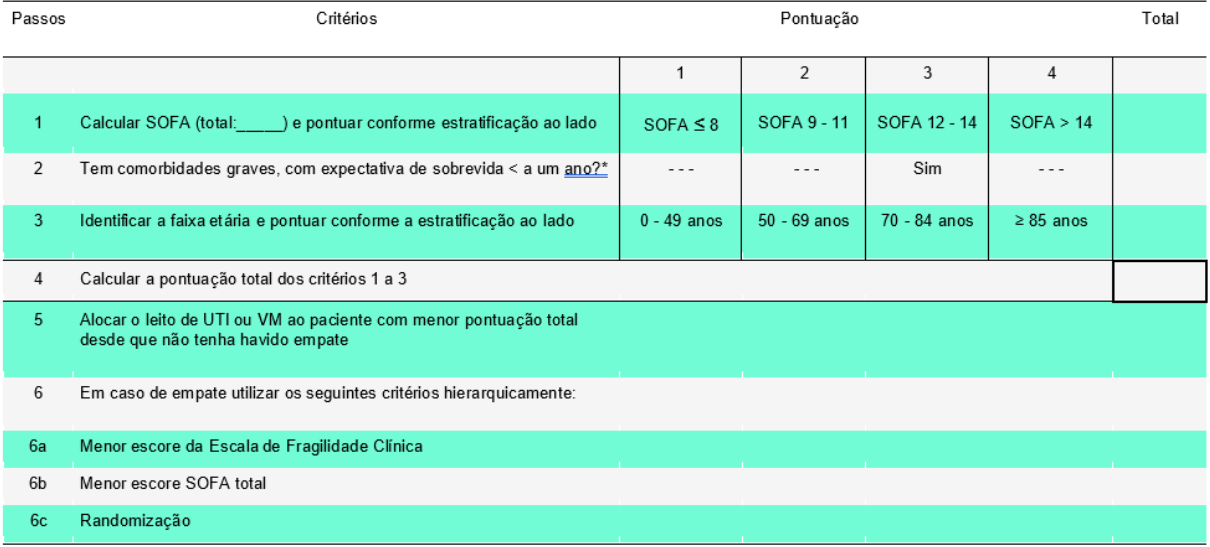
\includegraphics[scale=0.9]{img/Tabela de pontuacoes e criterios.png}
    \centering
    \caption{Calculo de pontuação e critério de desempate do modelo de triagem AMIB.}
    \label{subexpressao}
\end{figure}

O SOFA (abreviação para Sequential Sepsis-related Organ Failure Assessment), originalmente derivado de um estudo de coorte com 1449 pacientes internados em UTIs de 16 países nos anos 90, avalia objetivamente o avanço de uma disfunção orgânica em pacientes que apresentam alguma infecção, bem como a mortalidade diante de um estado de saúde crítico de um indivíduo.
O SOFA avalia 6 sistemas diferentes a partir de diversos exames clínicos e laboratoriais, e prediz a mortalidade de pacientes com sepse a partir da pontuação.

A tabela 1 demonstra a relação entre a pontuação no SOFA e a mortalidade:
PONTUAÇÃO SOFA	MORTALIDADE EM X%
0–6	<10\%
7–9	15–20\%
10–12	40–50\%
13–14	50–60\%
15	>80\%
15–24	>90\%

Esse score é baseado em seis diferentes variáveis, que avaliam os sistemas respiratório, cardiovascular, hepático, renal, neurológico e de coagulação. A cada sistema é atribuída uma pontuação de 0 (classificado como dentro dos parâmetros de normalidade) e 4 (alto grau de disfunção), totalizando um máximo de 24 pontos. A pontuação deve ser calculada 24 horas após a admissão e a cada 48 horas depois — justificando o termo “sequencial” do nome da pontuação.


SISTEMA RESPIRATÓRIO: é avaliado a partir da razão entre PaO2/FiO2, a partir de dados obtidos através de gasometria arterial. Essa razão é dada em milímetros de mercúrio (mmHg) e é considerada sem alterações quando seu valor está acima de 400mmHg. Abaixo de 400, 1 ponto no SOFA. Abaixo de 300, 2 pontos. A pontuação é 3 quando o paciente está em suporte ventilatório com a PaO2/FiO2 abaixo de 200, e ele recebe a pontuação máxima quando a relação tem resultado menor que 100mmHg com suporte ventilatório.

COAGULAÇÃO: é avaliada a partir do plaquetograma. O valor considerado de referência, ou seja, que não pontua no score SOFA, é 150.000/mm³. Os valores de corte para as pontuações de 1 a 4, respectivamente, são abaixo de 150, 100, 50 e 20. 

AVALIAÇÃO HEPÁTICA: realizada com o exame de bilirrubinas totais, que é considerado dentro dos valores de normalidade quando está abaixo de 1,2mg/dL.

SISTEMA CARDIOVASCULAR: o paciente que apresenta hipotensão e necessidade de droga vasoativa (DVA) é quem pontua nesta parte do score. É mensurado a partir da pressão arterial média, que recebe 1 ponto em caso de PAM<70mmHg. A partir do 2º ponto, é considerado o uso de DVA – 2 pontos se uso de dopamina<5 ou dobutamina em qualquer dose;  3 pontos em caso de uso de dopamina, noradrenalina ou adrenalina em doses mais baixas, e em caso de aumento da dosagem das DVAs, o paciente recebe a pontuação de 4 pontos.

SISTEMA NEUROLÓGICO: recebe avaliação a partir da escala de coma de Glasgow, conforme tabela 2. 
SISTEMA RENAL: é avaliado por dois parâmetros – creatinina e o débito urinário (a partir de 3 pontos). A creatinina se demonstra alterada a partir de 1,2mg/dL, pontuando 1 até 1,9mg/dL. Valores de 2,0 a 3,4mg/dL pontuam 2, enquanto o paciente que apresenta diurese menor que 500 ml por dia OU creatinina de 3,5 a 4,9mg/dL pontua 3. Quando a diurese é inferior a 200 ml por dia ou a creatinina é superior a 5, o paciente recebe o score máximo. 



\section{MODELO COMPUTACIONAL}

O roteiro do código se baseará no protocolo da Associação de Medicina Intensiva Brasileira (AMIB), de alocação de recursos em esgotamento durante a pandemia por COVID-19, pois entende-se que esse protocolo pode se estender para os dias pós pandemia. O protocolo busca um alinhamento com os critérios da resolução que priorizam a maior necessidade, expectativa de benefícios e adota a recomendação de que pacientes com baixa prioridade e que estão próximos à morte recebam preferencialmente cuidados paliativos. O protocolo AMIB contribui com a aplicação da resolução na medida que oferece critérios mais objetivos de avaliação de benefícios, aliviando o profissional do peso dessa tarefa em tempos de pandemia e garantindo que elas tenham maior consistência.
O modelo usará as variáveis extraídas do protocolo AMIB, sendo elas parte do Escore de falência de órgãos (protocolo Sequential Organ Failure Assessment - SOFA), com o objetivo de levantar e ensinar para o modelo quais os fatores de risco para a vida do paciente.

Considerando o protocolo AMIB, existem nove critérios clinicos a serem havaliados para a tomada de decisão, denotados $a_1$ até $a_9$:

\[
    \begin{split}
        a_1 &\in \mathbb{Z}; 20 \ge a_1 \ge 85\text{, sendo a idade do paciente} \\
        a_2 &\in \{0, 1, 2, 3, 4\}\text{, sendo o critério neurológico} \\
        a_3 &\in \{0, 1, 2, 3, 4\}\text{, sendo o critério respiratório} \\
        a_4 &\in \{0, 1, 2, 3, 4\}\text{, sendo o critério cardio-vascular} \\
        a_5 &\in \{0, 1, 2, 3, 4\}\text{, sendo o critério coagulatório} \\
        a_6 &\in \{0, 1, 2, 3, 4\}\text{, sendo o critério hepático} \\
        a_7 &\in \{0, 1, 2, 3, 4\}\text{, sendo o critério renal} \\
        a_8 &\in \{0, 3\}\text{, sendo o critério de comorbidades (ICC)} \\
        a_9 &\in \{0, 1, 2, 3, 4\}; a_1 < 60 \implies a_8=0\text{, sendo o critério oncológico (ECOG)} \\
    \end{split}
\] 

Notadamente, o protocolo não limita a idade para apeneas as faixas descritas, o procolo é aplicável para situações conde há pacientes com menos de vinte anos ou com mais de oitenta e cinco.
Essa restrição de idade foi decidida em prol da geração de dados, e poderia ser modificada.
Outra observação que de deve ressaltar é de que o critério oncológico é sujeito, no protocolo AMIB, à idade do paciente, isso é, mesmo com indicação clínica de tumores, o critério só os considera para pacientes com mais de sessenta anos.

Para a execução do protocolo são utilizadas as seguintes somas:

\[
\begin{split}
    s &= \sum_{n=2}^{7} a_n\text{, sendo o SOFA} \\
    t_1 &=  \begin{cases}
        1, \text{se } & a_1 \le 49 \\
        2, \text{se } 49 < & a_1 \le 69 \\
        3, \text{se } 69 < & a_1 \le 84 \\
        4, \text{se } 85 < & a_1 \\
    \end{cases} \\
    t_2 &= \begin{cases}
        1, \text{se } & s \le 8 \\
        2, \text{se } 8 < & s \le 11 \\
        3, \text{se } 11 < & s \le  14 \\
        4, \text{se } 14 < & s \\
    \end{cases} \\
    t &= t_1 + t_2 + a_8 + a_9 \\ % TODO revisar a soma
\end{split}
\] 

Dados dois pacientes, $p_1$ e $p_2$, o protocolo decide entre os dois primeiramente comparando o valor de $t$ calculado para cada um, se  $t_{p_1}$ for menor que $t_{p_2}$ o protocolo prescreve que a preferência na obtenção do leito seja de  $p_1.$
A reciproca, naturalmente, é verdadeira.
No caso de $t$ ser igual para os dois pacientes, é realizada a comparação usando  $s$. 
No caso de $t$ e de  $s$ serem iguais para os pacientes, utiliza-se o EU JÁ NEM ME LEMBRO MAIS.

Notadamente, é possível desenhar dois pacientes para que o protocolo seja incapaz de fornecer distinção relevante a respeito de priorização de um em relação a outro, no caso em que o protocolo sugere randomização.
Mais especificamente, é possível desenhar uma função $\alpha \in [0, 1]$ que informe o grau de certeza com o qual o protocolo determina a prioridade.

\[
\alpha = \begin{cases}
    \frac{t_{p_1} - t_{p_2}}{\max_t - \min_t}, \text{se } t_{p_1} - t_{p_2} \neq 0 \\
    \frac{a_{8p_1} - a_{8p_2}}{\max_{a_8} - \min_{a_8}}, \text{se } a_{8p_1} - a_{8p_2} \neq 0 \\
    \frac{s_{p_1} - s_{p_2}}{\max_s - \min_s}, \text{se } s_{p_1} - s_{p_2} \neq 0 \\
    0, \text{se o protocolo prescreve randomização}
\end{cases}
\] 

Sendo um objetivo minimizar $\alpha$, é preciso destavar de que isso é trivial considerando o caso de dois pacientes com todos os critérios idênticos, mas esse caso foge do que é desejável, pois não são cabíveis quaisquer outros argumentos quanto a priorização.
Para tando, se utiliza-se a noção de inercia ($i$) como medida de homogeneitdade, de forma que valores menores de $i$ implicam conjuntos de paciêntes mais homogêneos.
A inércia pode ser calculada como o quadrado da disância de cada menbro do conjunto para o centro de gravidade do conjunto.

\[
I = \sum_{p \in P}d(p, c)^2
\] 

Considerando $P$ o conjunto de pacientes, $c$ o centro de massa desse conjunto e $d$ a distância euclideana.

Com essas definições, é possível a construção de um conjunto de dados que maximize a obtenção de quais os critérios de decisão de um médico, presumindo que ele se informe pelo protocolo AMIB, mas que tome uma decisão médica para os casos em que o protocolo prescreve randomização.
Para tanto, qualquer que seja o conjunto de pacientes que o médico ordenará, esse deve maximizar a inercia e minimizar alfa.

Considerando uma função de qualidade $\frac{I}{\alpha}$, realiza-se uma busca por um conjunto de dez pacientes da seguintes forma:

É construído um novo paciente $P$ escolhendo um ponto nesse espaço de nove dimensões, nesse processo são feitas validações de $a_1$ até $a_9$ de forma que pertence aos conjuntos definidos. 
Também são validadas asa seguintes regras clínicas:

\[
\begin{split}
    R_1: a_4 \ge 3 \implies a_2 \ge 3 \\
    R_2: \ldots
\end{split}
\]

É construído um conjunto de 10 pacientes, para o conjunto é calculada a função $\frac{I}{\alpha}$.
É calculada a mesma função para os 10 subconjuntos de 9 elementos.
No subconjunto com maior $\frac{I}{\alpha}$ será complementado com um novo paciente gerado e validado se o $\frac{I}{\alpha}$ ainda é maior $\frac{I}{\alpha}$ do conjunto original.
Para a próxima etapa é utilizado qual dos dois conjuntos tiverem maior valor.
Esse processo se repete dez mil vezes.

isso fornece um conjunto de paciente homogêneos e em que o protocolo AMIB falha em prescrever qual paciente deve receber prioridade. 


\section{RESULTADOS EXPERIMENTAIS}


MÉDIA DOS CRITÉRIOS. ( IDADE (SOMA DO SOMA) ...

GRÁFICO DE DISPERSÃO...





\section{CONSIDERAÇÕES FINAIS}

Nóiz é F0d@

\section{PRÓXIMAS ETAPAS}

Interessante usar colapso de função de onda \ldots

Algoritmo genético para geração \ldots


\section{REFERÊNCIAS BIBLIOGRÁFICAS}

\bibliographystyle{sbc}
\bibliography{sbc-template}

\end{document}

